\documentclass[12pt, compress]{beamer}
\usetheme{m}

\usepackage{booktabs}
\usepackage[scale=2]{ccicons}

\usepgfplotslibrary{dateplot}

\title{Realization of a network stack that supports TAKS+WIDS on WSN with Mote Runner}
\subtitle{}
\date{\today}
\author{Andrea Salini - 231413\\Lorenzo Di Giuseppe - 227515\\Matteo Gentile - 230997}
\institute{DISIM - Università degli Studi dell’Aquila}

\begin{document}

  \maketitle
  
\begin{frame}[fragile]
  \frametitle{Introduction}
  \begin{itemize}
    \item Object of this project is the exploration of Mote Runner, an IBM’s infrastructure platform for WSN
    \item For a deep understanding of MR the focus of this works was the design and develop of a 802.15.4-like MAC layer
    \item The application was tested on IRIS mote
  \end{itemize}
\end{frame}

\begin{frame}[fragile]
  \frametitle{Index}
  \begin{itemize}
    \item Introduction to Mote Runner
    \item Testing Mote Runner
    \item A MAC Layer in Mote Runner
    \item ...
  \end{itemize}
\end{frame}

\section{Introduction to Mote Runner}
\begin{frame}[fragile]
  \frametitle{Mote Runner}
  \begin{itemize}
    \item An OS and a runtime and development environment for WSN
    \item Key features:
    \begin{itemize}
      \item Support for RT constraints \& energy awareness
      \item Portability thanks to a VM that abstracts the HW
      \item Event oriented programming paradigm
      \item High level coding (Java - C\#)
      \item Debugging \& simulation environments
    \end{itemize}
    \item It’s still in beta and is evolving towards IoT
  \end{itemize}
\end{frame}

\begin{frame}[fragile]
  \frametitle{Mote Runner}
  \begin{columns}
    \begin{column}{.48\linewidth}
    	
    \end{column}
    \hfill
    \begin{column}{.5\linewidth}
    	\begin{figure}
	  \centering
	  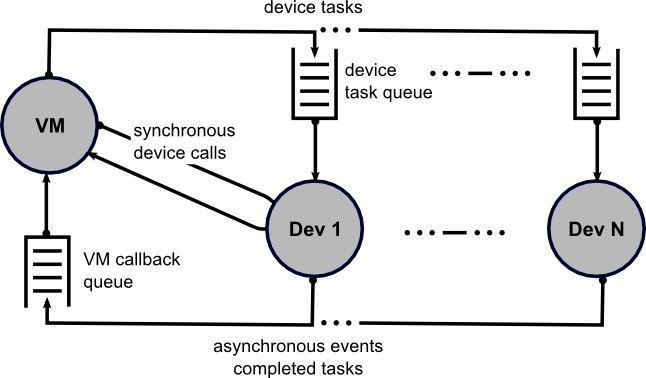
\includegraphics[width=\textwidth]{img/vm-dev.jpg}
    	\end{figure}
    \end{column}
  \end{columns}
\end{frame}

\begin{frame}[fragile]
  \frametitle{Mote Runner}
  \begin{columns}
    \begin{column}{.5\linewidth}
    	\begin{figure}
	  \centering
	  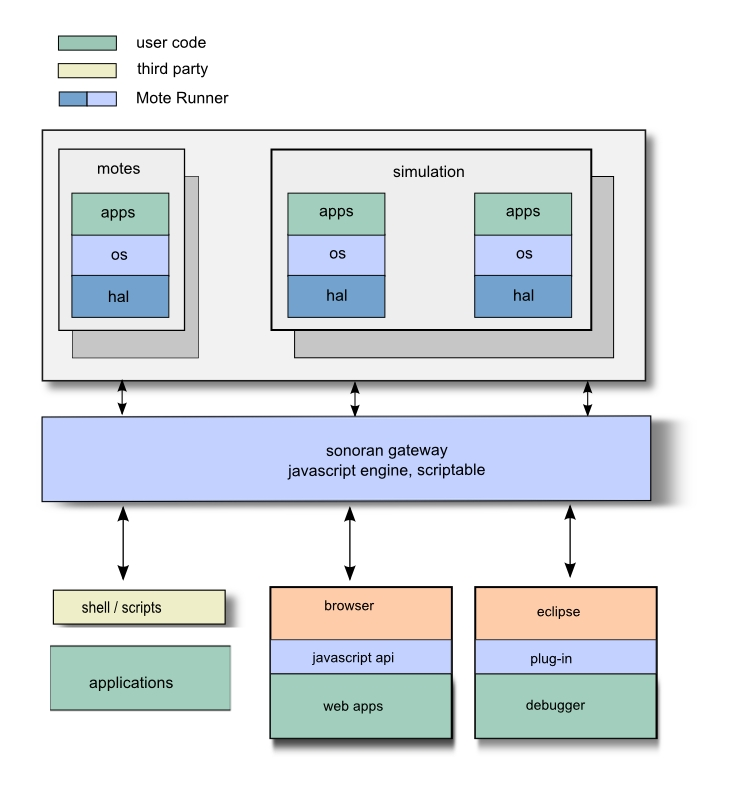
\includegraphics[width=\textwidth]{img/overview.jpg}
    	\end{figure}
    \end{column}
    \hfill
    \begin{column}{.5\linewidth}
    	\begin{figure}
	  \centering
	  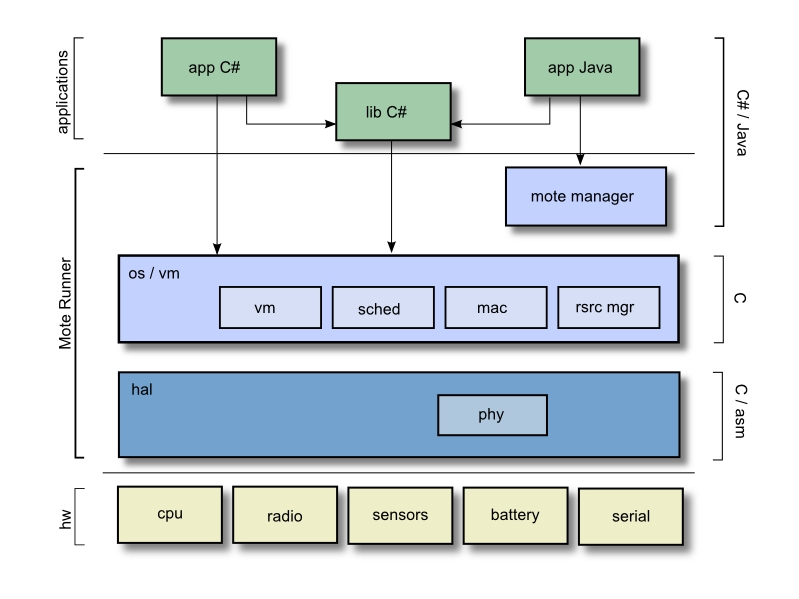
\includegraphics[width=\textwidth]{img/onmote.jpg}
    	\end{figure}
    \end{column}
  \end{columns}
\end{frame}

\begin{frame}[fragile]
  \frametitle{Mote Runner - v.11, v.13 beta}
  \begin{itemize}
    \item They support IEEE 802.15.4
    \begin{itemize}
    	\item exposing a low radio level API that can be used to implement custom MAC layer
    	\item dropping messages with header structure not 802.15.4 compliant in the radio stack 
    \end{itemize}
    \item Offer Hopi
    \begin{itemize}
    	\item A multi-hop data gathering protocol
    	\item Used to collect data from motes setting automatically a tree network
    \end{itemize}
  \end{itemize}
\end{frame}

\begin{frame}[fragile]
  \frametitle{Mote Runner - v.17.1.8c (latest)}
  \begin{itemize}
    \item Supports only two platforms: IMST \& Blipper
    \item It’s based on a different radio layer: LoRa\texttrademark
    \item It offers a build-in MAC layer: LRSC - Low Range Signaling \& Control
    \begin{itemize}
    	\item It supports only a network topology: the LRSC one
    	\item The offered API is poor since the radio is hidden in the firmware (not compatible with previous versions)
    \end{itemize}

  \end{itemize}
\end{frame}

\begin{frame}[fragile]
  \frametitle{LRSC - Architecture}
  \begin{columns}
    \begin{column}{.48\linewidth}
    	\begin{itemize}
	  \item Gateways (GW) are connected to server on IP
	  \item Motes comunicate with server in tunneling TCP/UDP over IP
	  \item Motes comunicate with GW with LoRa single-hop
    	\end{itemize}
    \end{column}
    \hfill
    \begin{column}{.48\linewidth}
    	\begin{figure}
	  \centering
	  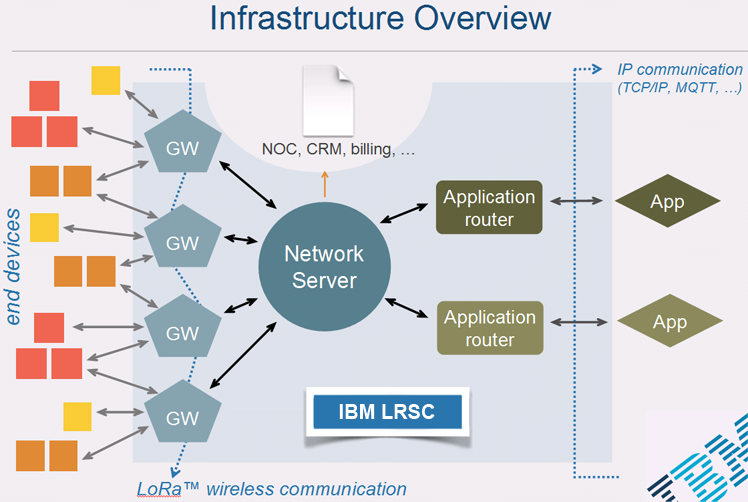
\includegraphics[width=\linewidth]{img/LRSC_infrastructure.png}
    	\end{figure}

    \end{column}
  \end{columns}
\end{frame}

\begin{frame}[fragile]
  \frametitle{LoRa\texttrademark}
  \begin{columns}
    \begin{column}{.48\linewidth}
      \begin{itemize}
	\item LoRa\texttrademark Alliance
	\begin{itemize}
	  \item Target: IoT,  machine-to-machine (M2M), smart city, and industrial applications
	  \item Intiated to standardize Low Power Wide Area Networks (LPWAN)
	\end{itemize}
      \end{itemize}
    \end{column}
    \hfill
    \begin{column}{.48\linewidth}
    	\begin{figure}
	  \centering
	  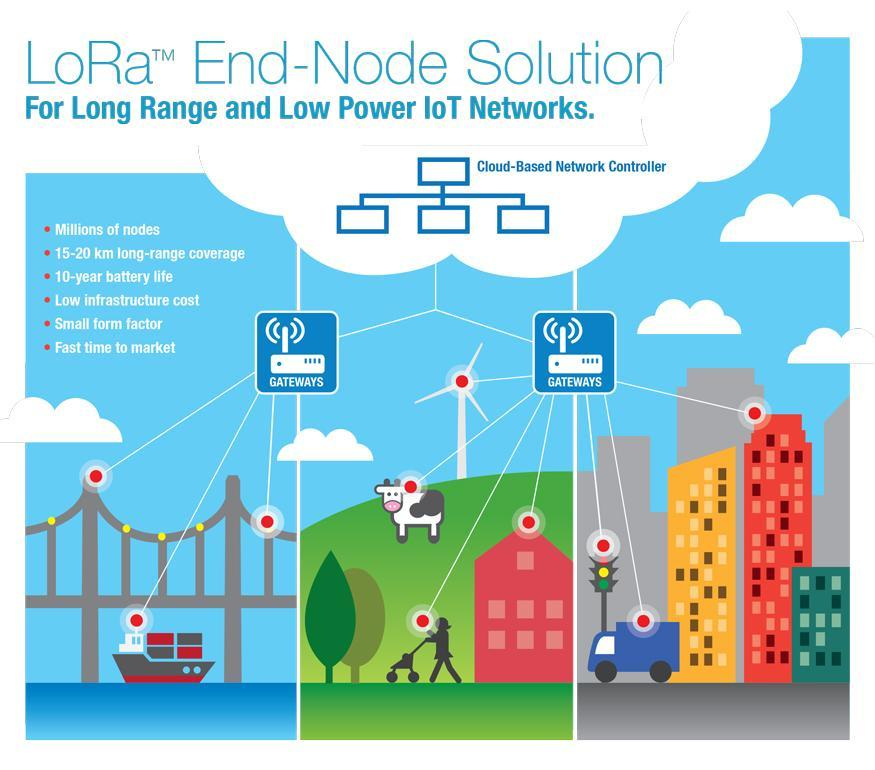
\includegraphics[width=\linewidth]{img/lora.jpg}
    	\end{figure}

    \end{column}
  \end{columns}
\end{frame}

\begin{frame}[fragile]
  \frametitle{LoRa\texttrademark}
  \begin{itemize}
    \item LoRa\texttrademark Technology
    \begin{itemize}
      \item LoRaWAN pledeges to extend the radio range by 10x while using only one third of the power used by competing solutions 
      \item Star (of stars?) topology
      \item Gateways relay messages between end-devices and a central network server
      \item Communication between end-devices and gateways is spread out on different frequency channels and data rates.
      \item Data rates: 0.3 - 50 kbps
    \end{itemize}
  \end{itemize}
\end{frame}

\begin{frame}[fragile]
  \frametitle{LoRa\texttrademark}
  \begin{itemize}
    \item ...and more
    \begin{itemize}
      \item adaptive data rate (ADR)
      \item secure communication (on network and application layers and end-point device key)
      \item three classes of end-point devices.
      \item More info on http://lora-alliance.org/
    \end{itemize}
  \end{itemize}
\end{frame}

\begin{frame}[fragile]
  \frametitle{Mote Runner - Conclusion}
  \vspace{-1em}
  \begin{itemize}
    \item For the purpose of this work (TAKS \& WIDS):
    \begin{itemize}
    	\item MR allows dynamic reprogramming of motes with a control server using WLIP
    	\item v.17.1.8c is not suitable
    	\begin{itemize}
	  \item LoRa is available only for a limited number of platforms (until now!)
	  \item LRSC doesn’t permit to customize the MAC behaviour
	  \item The radio is not exposed
    	\end{itemize}
    	\item v.11, v.13 are better choices:
    	\begin{itemize}
	  \item radio interface could be used to implement an 802.15.4 MAC with TAKS support
	  \item this MAC could be used to build upper layer with WIDS
    	\end{itemize}
    \end{itemize}
    \item This does not exclude a future integration with LoRa-LRSC
  \end{itemize}
\end{frame}

\begin{frame}[fragile]
  \frametitle{Mote Runner}
  \begin{itemize}
  	\item 
  \end{itemize}
\end{frame}
\section{Physical layer in \mbox{Mote Runner}}
\begin{frame}[fragile]
  \frametitle{Radio interface - 1}
  \begin{itemize}
    \item MR v.13 offers a Radio interface IEEE 802.15.4 compliant
    \begin{itemize}
    	\item It is a generic class in the IBM saguaro system that permits to use the radio device
    	\item It offers an API with the following functionality:
    	\begin{itemize}
			\item open: opens the radio, once opened no other assembly can use it
			\item close: releases the radio so that others can use it
			\item setter and getters for channel and network parameters (addresses, panid...)
			\item startReceive: listens the channel (in one of the many receiption mode)
			\item transmit: begin to transmit a pdu
    	\end{itemize}
    \end{itemize}
  \end{itemize}
\end{frame}

\begin{frame}[fragile]
	\frametitle{Radio interface - 2}
	\begin{itemize}
		\item In addition Radio:
		\begin{itemize}
			\item Handles transmission and reception notifying to higher level by delegation, registering functions that will handle the events (tx and rx)
			\item Manages acks notifying states of failure or success to callbacks
			\item Permits to set parameters as PAN identifier, short address, radio channel
		\end{itemize}
	\end{itemize}
\end{frame}


\begin{frame}[fragile]
  \frametitle{Transmission \& Reception - 1}
  \begin{itemize}
    \item These operations require much attention:
    \begin{itemize}
    	\item Radio permits to transmit every type of pdu, but it's possible to receive only packets with 802.15.4 well formed headers
    	\item Receiving in promiscuous mode allows to receive every kind of packet, but this exposes to interferences
    \end{itemize}
    \item Each mote holds 3 addresses:
    \begin{itemize}
    	\item a 16-bit PAN identifier
    	\item a 64-bit extended address that uniquely identifies a mote (EUI-64)
    	\item a 16-bit short address that's application and protocol specific
    \end{itemize}
  \end{itemize}
\end{frame}

\begin{frame}[fragile]
  \frametitle{Transmission \& Reception - 2}
  \begin{figure}
  	\centering
  	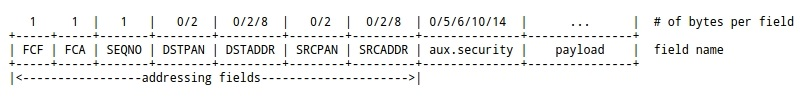
\includegraphics[width=\textwidth]{img/header.jpg}
  	\caption{PDU header format}
  \end{figure}
  \begin{columns}
  	\begin{column}{.52\textwidth}
	    \begin{figure}
	    	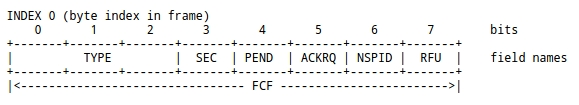
\includegraphics[width=\textwidth]{img/fcf.jpg}
  		\caption{Frame Control Flags}
	    \end{figure}
  	\end{column}
  	\hfill
	\begin{column}{.45\textwidth}
	    \begin{figure}
	    	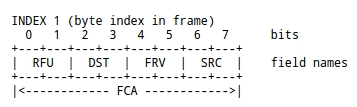
\includegraphics[width=\textwidth]{img/fca.jpg}
  		\caption{Frame Control Address Flags}
	    \end{figure}
  	\end{column}
  \end{columns}
\end{frame}
% 
% \begin{frame}[fragile]
%   \frametitle{Tx/Rx - Filtering}
%   \begin{itemize}
%     \item Possible packets are specified in FCF-Type field and are: BEACON, DATA, ACK and CMD.
%     \item BEACONs are accepted only if the header field SRCPAN matches the mote's PANID or it's BROADCAST
%     \item If FCA Flags specify an address then 
%   \end{itemize}
% \end{frame}

\begin{frame}[fragile]
  \frametitle{Tx/Rx and Real Time Constraints}
  \begin{itemize}
    \item It's possible to operate in many different ways with regards to real time constraints:
    \begin{itemize}
    	\item ASAP, EXACT, TIMED, RX4EVER indicate when the operation should begin and/or end given two time instant
    	\item MR manages autonomously all warm up and ramp up to make the device ready given one of these modes
    	\item At the end the device turns off and an event is raised to be managed with delegation
    	\item If the device cannot be ready or cannot complete a task within the specified time an error occurs
    \end{itemize}
  \end{itemize}
\end{frame}
\section{A MAC Layer in Mote Runner}
\begin{frame}[fragile]
  \frametitle{Coming soon}
  
\end{frame}
\section{Conclusions} 
\begin{frame}[fragile]
  \frametitle{TODO}
\end{frame}


\end{document}
